\documentclass[12pt]{article}
\usepackage{amsmath} % for mathematical formulas
\usepackage{amssymb} % for mathematical symbols
\usepackage{tikz} % for creating diagrams
\usetikzlibrary{shapes.geometric, arrows.meta, bending}
\usepackage{graphicx} % for including images
\usepackage{geometry} % for adjusting margins
\geometry{a4paper, margin=1in}

\title{Introduction to Angular Momentum, Work, and Power in Rotational Motion}
\author{Your Name}
\date{\today}

\begin{document}

\maketitle

\section{Introduction}
Angular momentum is a fundamental concept in physics that describes the motion of objects in rotational movement. It is particularly important in systems involving circular motion and is conserved in isolated systems, making it a powerful tool in analyzing physical phenomena.

\section{Definition of Angular Momentum}
Angular momentum, \(\vec{L}\), of a particle about a point is defined as the cross product of the particle's position vector, \(\vec{r}\), relative to the point, and its linear momentum, \(\vec{p}\):
\[
\vec{L} = \vec{r} \times \vec{p}
\]
where \(\vec{p} = m\vec{v}\) and \(m\) is the mass of the particle, and \(\vec{v}\) is its velocity.

\section{Conservation of Angular Momentum}
The angular momentum of a system remains constant if no external torques are acting on it. This principle can be expressed as:
\[
\frac{d\vec{L}}{dt} = \vec{\tau}
\]
where \(\vec{\tau}\) is the external torque applied to the system. In the absence of external torques, \(\vec{\tau} = 0\) and therefore \(\frac{d\vec{L}}{dt} = 0\), implying conservation of angular momentum.

\section{Applications of Angular Momentum}
\subsection{Astronomy}
The conservation of angular momentum explains why planets in our solar system rotate faster as they get closer to the sun in their elliptical orbits.
\subsection{Sports}
In figure skating, a skater pulls their arms in to spin faster on the ice. This is a practical demonstration of conservation of angular momentum.

\section{Kinematic Relationships in Rotational Motion}
\subsection{Linear Momentum and Angular Momentum}
Linear momentum \(\vec{p}\) of a body is defined as the product of its mass \(m\) and its velocity \(\vec{v}\):
\[
\vec{p} = m\vec{v}
\]
Angular momentum \(\vec{L}\) for a particle can be calculated using the position vector \(\vec{r}\) and the linear momentum \(\vec{p}\) as follows:
\[
\vec{L} = \vec{r} \times \vec{p} = r m \vec{v} \sin(\theta)
\]
where \(\theta\) is the angle between \(\vec{r}\) and \(\vec{v}\).

\subsection{Right-Hand Rule for Angular Momentum}
The direction of angular momentum is determined using the right-hand rule. Below is a diagram illustrating this rule:

\begin{figure}[h]
\centering
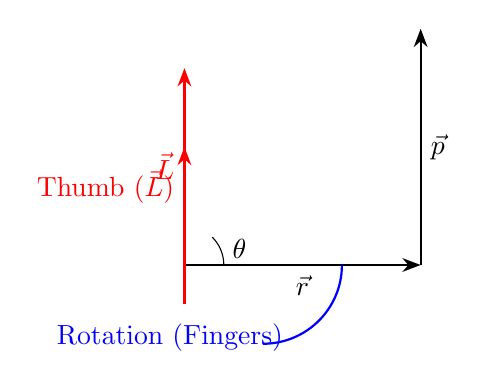
\begin{tikzpicture}
    % Define coordinates for the vectors
    \coordinate (O) at (0, 0);
    \coordinate (R) at (3, 0);
    \coordinate (P) at (3, 3);
    \coordinate (L) at (0, 2.5);

    % Draw vectors
    \draw[-Stealth, thick] (O) -- (R) node[midway, below] {$\vec{r}$}; % radial vector
    \draw[-Stealth, thick] (R) -- (P) node[midway, right] {$\vec{p}$}; % momentum vector
    \draw[-Stealth, thick, red] (O) -- (L) node[midway, left] {$\vec{L}$}; % angular momentum vector

    % Draw the arc for angle theta
    \draw (0.5, 0) arc[start angle=0, end angle=45, radius=0.5];
    \node at (0.7, 0.2) {$\theta$};

    % Illustrate the right-hand rule
    \draw[thick, blue] (1, -1) arc[start angle=270, end angle=360, radius=1] node[near start, left] {Rotation (Fingers)};
    \draw[thick, red, -Stealth] (0, -0.5) -- (0, 1.5) node[near end, left] {Thumb (\(\vec{L}\))};
\end{tikzpicture}
\caption{Applying the right-hand rule to determine the direction of angular momentum.}
\end{figure}

\section{Angular Velocity and Angular Acceleration}
Angular velocity \(\omega\) is defined as the rate of change of angular displacement and is given by:
\[
\omega = \frac{d\theta}{dt}
\]
where \(\theta\) is the angular displacement. Angular velocity is related to the linear velocity \(v\) by the equation:
\[
v = r \omega
\]
where \(r\) is the radius of the motion path.

Angular acceleration \(\alpha\) is defined as the rate of change of angular velocity:
\[
\alpha = \frac{d\omega}{dt}
\]
It describes how quickly the angular velocity changes over time. Angular acceleration is related to the tangential acceleration \(a_t\) by:
\[
a_t = r \alpha
\]

\section{Work and Power in Rotational Motion}
\subsection{Work Done by a Torque}
Work done by a torque in rotational motion is given by the integral of torque \(\tau\) with respect to angular displacement \(\theta\):
\[
W = \int \tau \, d\theta
\]
where \(\tau\) is the torque and \(\theta\) is the angle of rotation.

\subsection{Power in Rotational Systems}
Power in rotational motion is defined as the rate of doing work or the rate of change of angular energy:
\[
P = \frac{dW}{dt} = \tau \omega
\]
where \(P\) is the power, \(\tau\) is the torque, and \(\omega\) is the angular velocity. This relationship shows how effectively a rotating system can perform work over time.

\section{Common Moments of Inertia}

This section presents the moments of inertia for various standard geometries about their center of mass, unless otherwise noted. The moment of inertia (\(I\)) is a measure of an object's resistance to changes in its rotational motion.

\subsection{Point Mass}
For a point mass \(m\) at a distance \(r\) from the axis of rotation:
\[
I = mr^2
\]
\begin{figure}[h]
\centering
\begin{tikzpicture}
\filldraw[black] (0,0) circle (2pt) node[anchor=north] {\(m\)};
\draw[thick, dashed] (0,0) -- (2,0) node[midway, above] {\(r\)};
\draw[thick] (0, -1) -- (0, 1);
\end{tikzpicture}
\caption{Point mass at a distance \(r\) from the rotation axis.}
\end{figure}

\subsection{Solid Sphere}
For a solid sphere of radius \(R\) and mass \(m\):
\[
I = \frac{2}{5} mR^2
\]
\begin{figure}[h]
\centering
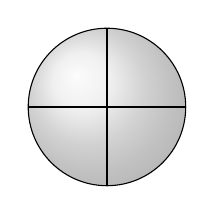
\begin{tikzpicture}
\shade[ball color = gray!40, opacity = 0.4] (0,0) circle (1cm);
\draw (0,0) circle (1cm);
\draw (-1,0) -- (1,0);
\draw (0,-1) -- (0,1);
\end{tikzpicture}
\caption{Solid sphere.}
\end{figure}

\subsection{Hollow Sphere}
For a thin-walled hollow sphere of radius \(R\) and mass \(m\):
\[
I = \frac{2}{3} mR^2
\]
\begin{figure}[h]
\centering
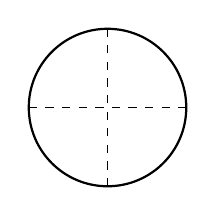
\begin{tikzpicture}
\draw[thick] (0,0) circle (1cm);
\draw[dashed] (-1,0) -- (1,0);
\draw[dashed] (0,-1) -- (0,1);
\end{tikzpicture}
\caption{Hollow sphere.}
\end{figure}

\subsection{Solid Cylinder}
For a solid cylinder of radius \(R\) and mass \(m\), about its axis:
\[
I = \frac{1}{2} mR^2
\]
\begin{figure}[h]
\centering
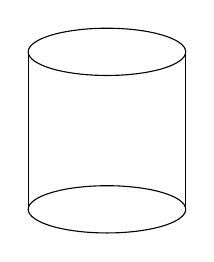
\begin{tikzpicture}
\draw (0,0) ellipse (1 and 0.3);
\draw (-1,0) -- (-1,-2);
\draw (1,0) -- (1,-2);
\draw (0,-2) ellipse (1 and 0.3);
\end{tikzpicture}
\caption{Solid cylinder.}
\end{figure}

\subsection{Hollow Cylinder}
For a hollow cylinder (thin-walled) of radius \(R\) and mass \(m\), about its axis:
\[
I = mR^2
\]
\begin{figure}[h]
\centering
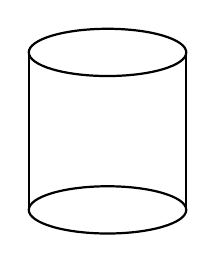
\begin{tikzpicture}
\draw[thick] (0,0) ellipse (1 and 0.3);
\draw[thick] (-1,0) -- (-1,-2);
\draw[thick] (1,0) -- (1,-2);
\draw[thick] (0,-2) ellipse (1 and 0.3);
\end{tikzpicture}
\caption{Hollow cylinder.}
\end{figure}

\subsection{Rectangular Plate}
For a rectangular plate of mass \(m\), height \(h\), and width \(w\), spinning around an axis through its center and perpendicular to the plate:
\[
I = \frac{1}{12} m(h^2 + w^2)
\]
\begin{figure}[h]
\centering
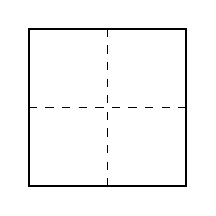
\begin{tikzpicture}
\draw[thick] (-1,1) rectangle (1,-1);
\draw[dashed] (0,1) -- (0,-1);
\draw[dashed] (-1,0) -- (1,0);
\end{tikzpicture}
\caption{Rectangular plate.}
\end{figure}

\subsection{Thin Rod}
For a thin rod of length \(L\) and mass \(m\), spinning around an axis through its center perpendicular to the length:
\[
I = \frac{1}{12} mL^2
\]
\begin{figure}[h]
\centering
\begin{tikzpicture}
\draw[thick] (0,0) -- (2,0);
\draw[dashed] (1,0.2) -- (1,-0.2);
\end{tikzpicture}
\caption{Thin rod.}
\end{figure}
\section{Rolling Motion}

Rolling motion is a type of motion that involves both translational and rotational movement of an object, such as a sphere. One of the key concepts in rolling motion is rolling without slipping, which occurs when the point of the object in contact with the ground does not slide.

\subsection{Condition for Rolling Without Slipping}
The condition for rolling without slipping is given by:
\[
v = r\omega
\]
where \(v\) is the translational velocity of the center of mass, \(r\) is the radius of the sphere, and \(\omega\) is the angular velocity. This relationship ensures that the linear velocity at the point of contact with the ground is zero.

\subsection{Kinetic Energy in Rolling Motion}
The total kinetic energy (\(K\)) of a rolling object is the sum of its translational kinetic energy and rotational kinetic energy:
\[
K = \frac{1}{2} mv^2 + \frac{1}{2} I\omega^2
\]
where \(m\) is the mass of the sphere, \(I\) is the moment of inertia about the axis of rotation (\(I = \frac{2}{5}mR^2\) for a solid sphere), and \(v\) and \(\omega\) are linked by the rolling without slipping condition.

\subsection{Illustration of Rolling Motion}
Below is a diagram illustrating a sphere rolling without slipping. The arrow indicates the direction of motion, while the rotation is shown with respect to the center of mass.

\begin{figure}[h]
\centering
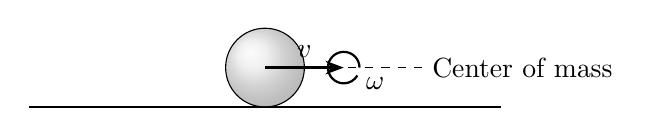
\begin{tikzpicture}
    % Ground
    \draw[thick] (-3,0) -- (3,0);
    % Sphere
    \shade[ball color = gray!40, opacity = 0.4] (0,0.5) circle (0.5);
    \draw (0,0.5) circle (0.5);
    % Axis through the center
    \draw[dashed] (0,0.5) -- (2,0.5) node[right] {Center of mass};
    % Direction of motion
    \draw[-Stealth, thick] (0,0.5) -- (1,0.5) node[above, midway] {\(v\)};
    % Rotation arrow
    \draw[thick] (1.2,0.5) arc (0:330:0.2);
    \node at (1.4,0.3) {\(\omega\)};
\end{tikzpicture}
\caption{A sphere rolling without slipping on a flat surface.}
\end{figure}

This section on rolling motion explains the dynamics of spherical objects like balls when they roll without slipping, integrating both translational and rotational aspects of motion. The diagram helps visualize the motion and the forces involved.

\section{Calculation of Moment of Inertia Using Integrals}

The moment of inertia (\(I\)) of an object about an axis is calculated by integrating the product of the square of the distance from the axis (\(r^2\)) and the mass density over the volume of the object. The general formula for moment of inertia is:
\[
I = \int r^2 \, dm
\]
where \(dm\) is the mass element and \(r\) is the distance from the axis of rotation to the mass element.

\subsection{Example: Moment of Inertia of a Disk}
Consider a uniform circular disk of radius \(R\) and mass \(M\), rotating about an axis through its center perpendicular to its face. The moment of inertia can be calculated by:
\[
I = \int_0^R \int_0^{2\pi} r^3 \rho \, d\theta \, dr
\]
where \(r\) is the radial distance from the axis, \(\theta\) is the angular coordinate, and \(\rho = \frac{M}{\pi R^2}\) is the mass per unit area. Simplifying, we find:
\[
I = \frac{1}{2} MR^2
\]
This calculation involves setting up an integral over the disk's area, multiplying each infinitesimal mass element by the square of its distance from the axis of rotation.

\subsection{Visual Representation}
Below is a diagram illustrating the division of a disk into infinitesimal elements for integration:

\begin{figure}[h]
\centering
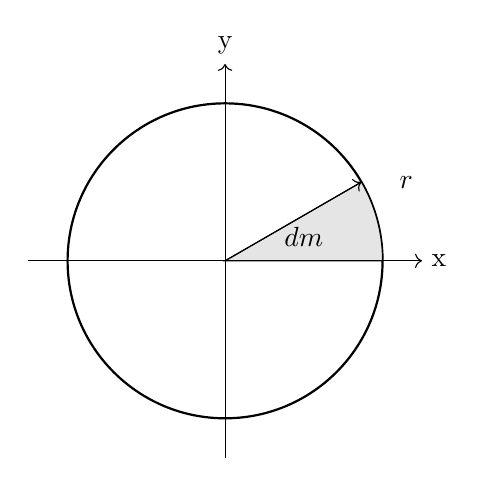
\begin{tikzpicture}
    % Draw the disk
    \draw[thick] (0,0) circle (2);
    \filldraw[fill=gray!20] (0,0) -- (2,0) arc[start angle=0,end angle=30,radius=2] -- cycle;
    \draw[->] (-2.5,0) -- (2.5,0) node[right] {x};
    \draw[->] (0,-2.5) -- (0,2.5) node[above] {y};
    \node at (1, 0.3) {\(dm\)};
    \node at (2.3, 1) {\(r\)};
    \draw[->] (0,0) -- (1.73, 1); % r vector
\end{tikzpicture}
\caption{Division of a disk into differential mass elements for calculating moment of inertia.}
\end{figure}

\section{Torque}

Torque (\(\vec{\tau}\)) is a measure of the force causing the rotation of an object about an axis. It is defined as the cross product of the position vector (\(\vec{r}\)) and the force vector (\(\vec{F}\)), leading to:
\[
\vec{\tau} = \vec{r} \times \vec{F}
\]
The magnitude of torque depends on three factors: the magnitude of the force, the distance of the force from the axis of rotation (lever arm), and the angle between the position vector and the force vector.

\subsection{Example: Torque on a Door}
If a force is applied perpendicularly at the edge of a door, the torque is maximized, as the lever arm is equal to the distance from the hinge to the point where the force is applied. The torque can be calculated by:
\[
\tau = rF
\]
where \(r\) is the distance from the hinge to the point of application of the force, and \(F\) is the force applied.

\subsection{Illustration of Torque}
Below is a diagram showing how torque is applied to a door:

\begin{figure}[h]
\centering
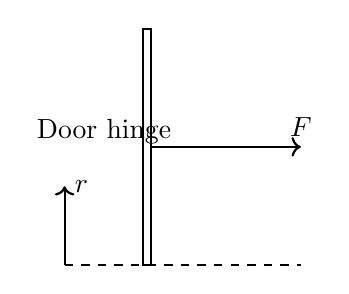
\begin{tikzpicture}
    % Draw the door
    \draw[thick] (0,0) rectangle (0.1,3);
    \draw[thick, ->] (0.1,1.5) -- (2,1.5) node[above] {\(F\)};
    \draw[dashed] (-1,0) -- (2,0);
    \draw[thick, ->] (-1,0) -- (-1,1) node[right] {\(r\)};
    \node at (-0.5,1.7) {Door hinge};
\end{tikzpicture}
\caption{Application of force at the edge of a door to create torque.}
\end{figure}


\end{document}
